\documentclass[a4paper, 10pt, titlepage]{report}

% --- PACKAGES ---
\usepackage[T5]{fontenc}
\usepackage[utf8]{inputenc}
\usepackage[english]{babel}
\usepackage{geometry}
\geometry{top=2.5cm, bottom=2.5cm, left=2cm, right=2cm}
\usepackage{amsmath}
\usepackage{amssymb}
\usepackage{algorithm}
\usepackage{algpseudocode}
\usepackage{graphicx}
\usepackage{float}
\usepackage{hyperref}
\usepackage{enumitem}
\usepackage{fancyhdr}
\usepackage{xcolor}
\usepackage[most]{tcolorbox}
\usepackage{array}
\usepackage{amsmath}
\usepackage{tikz}
\usepackage{tcolorbox}

% --- BOX STYLE ---
\tcbset{
    myhbox/.style={
        enhanced, 
        breakable,
        colback=white,
        colframe=blue!30!black,
        attach boxed title to top left={yshift*=-\tcboxedtitleheight}, 
        boxed title size=title,
        boxed title style={
            sharp corners, 
            rounded corners=northwest, 
            colback=blue!30!black, 
            boxrule=0pt,
        },
        underlay boxed title={
            \path[fill=blue!30!black] (title.south west)--(title.south east) 
            to[out=0, in=180] ([xshift=5mm]title.east)--
            (title.center-|frame.east)
            [rounded corners=3pt] |- 
            (frame.north) -| cycle; 
        }
    }
}

\newtcolorbox{featurebox}[1]{
    myhbox,
    title={#1}
}

% --- HEADER & FOOTER ---
\pagestyle{fancy}
\fancyhf{}
\lhead{\textbf{Project Report}}
\rhead{\textbf{R-Tree Spatial Indexing}}
\cfoot{\thepage}

\begin{document}

% ==============================================================================
% TITLE PAGE
% ==============================================================================
\begin{titlepage}
    \begin{center}
        \vspace*{1cm}
        
        \large
        \textbf{VIETNAM NATIONAL UNIVERSITY, HO CHI MINH CITY}\\
        \vspace{0.2cm}
        \textbf{UNIVERSITY OF SCIENCE --- VNUHCM}\\
        \vspace{0.2cm}
        \textbf{Faculty of Information Technology}
        
        \vspace{3cm}
        
        \Large
        \textbf{PROJECT REPORT --- R-TREE SPATIAL INDEXING}

        \large
        \vspace{0.2cm}
        (Final Version)
        
        \vspace{0.5cm}
        \LARGE
        \textit{Subject: CS163 - Data Structures and Algorithms}
        
        \vspace{1.5cm}
        
        \begin{table}[h]
            \centering
            \large
            \begin{tabular}{ll}
                \textbf{Group:}      & 51 \\
                \textbf{Class:}   & 25A02 \\
                \textbf{Submission Date:} & \today \\
            \end{tabular}
        \end{table}

        \vspace{1.0cm}

        \begin{figure}[H] 
        \centering
        
\includegraphics[width=0.3\textwidth]{hcmus-logo.png} 
        \end{figure}

        \vfill
        \textbf{Ho Chi Minh City, 2026}
    \end{center}
\end{titlepage}

\newpage
% ==============================================================================
% 1. PROGRAMMING ASSIGNMENTS
% ==============================================================================

\tableofcontents

\chapter{Fundamentals of the R-Tree}

\section{Introduction and Historical Context}
The R-tree is a hierarchical, multidimensional indexing structure specifically designed to manage spatial data such as points, line segments, and polygons. Introduced by Antonin Guttman of the University of California, Berkeley, in 1984, the R-tree serves as a multidimensional extension of the B-tree (specifically the B+ tree variant). While traditional indexing structures are optimized for one-dimensional data, the R-tree excels in processing window queries or orthogonal range reporting, making it a cornerstone of modern Geographic Information Systems (GIS) and spatial databases.

\section{Structural Characteristics}

\subsection{Balance and Symmetry}
Mirroring the properties of B-trees, R-trees are perfectly height-balanced, ensuring that all leaf nodes reside at the same level. This balance is maintained dynamically through specific occupancy rules governed by a parameter $B$, representing the maximum node capacity.

\subsection{Node Capacity and Occupancy Rules}
For an R-tree of order $B$ (where $B \ge 3$), the following constraints apply to maintain tree density and search efficiency:
\begin{itemize}
    \item \textbf{Leaf Nodes:} Each leaf contains between $0.4B$ and $B$ data objects. The only exception is the root, which may contain between $1$ and $B$ objects.
    \item \textbf{Internal Nodes:} Each internal node possesses between $0.4B$ and $B$ children. If the root is an internal node, it must have at least $2$ children.
\end{itemize}
In disk-resident implementations, $B$ is typically chosen so that a node's size corresponds to a single disk block, minimizing I/O overhead.

\subsection{Minimum Bounding Rectangles (MBR)}
The fundamental unit of spatial organization in an R-tree is the Minimum Bounding Rectangle (MBR). For any node $u$, let $S_u$ be the set of all spatial objects within its subtree. An internal node $u$ with children $v_1, v_2, \dots, v_f$ (where $f \le B$) stores an entry for each child consisting of:
\begin{enumerate}
    \item A pointer to the child node $v_i$
    \item $MBR(v_i)$, the smallest axis-parallel rectangle that tightly encloses all objects in the subtree $S_{v_i}$
\end{enumerate}





\section{Optimization Principles in Construction}
The R-tree definition does not strictly dictate how objects should be grouped into nodes. However, the quality of grouping significantly impacts performance.

\subsection{Perimeter vs. Area Minimization}
A core heuristic in R-tree construction is the minimization of the \textbf{perimeter sum} of all MBRs rather than their total area. 
\begin{itemize}
    \item \textbf{Query Efficiency:} Rectangles with smaller perimeters tend to be more square-like, reducing the probability of overlap with other MBRs or the query window $q$.
    \item \textbf{Geometric Logic:} While minimizing perimeter often minimizes area, the inverse is not always true. A rectangle can have a very small area but a large perimeter (e.g., a long, thin "needle" shape. Such shapes are inefficient for spatial indexing as they are more likely to intersect search regions across large distances.
\end{itemize}



\subsection{The Filter-Refinement Framework}
In complex applications like road segment retrieval, the R-tree is often used within a Filter-Refinement framework:
\begin{enumerate}
    \item \textbf{Filter Step:} The R-tree quickly identifies a \textit{Candidate Set} of MBRs that intersect the query window. This step is ($\mathcal{O}(\log N + k)$), but may include False Hits.
    \item \textbf{Refinement Step:} A secondary geometric check is performed on the candidate set to determine if the actual spatial object (e.g., a diagonal line) truly intersects the query window.
\end{enumerate}

\chapter{Algorithms}

This chapter analyzes the core algorithms that maintain the R-tree’s structural integrity and facilitate efficient multidimensional data retrieval. These mechanisms include spatial searching, point insertion, deletion and node splitting.

\section{2D Orthogonal Range Reporting (Window Query)}
The primary operation supported by the R-tree is 2D Orthogonal Range Reporting, or a window query. This is essential for applications requiring data retrieval within specific geographic or attribute-defined boundaries, such as map displays.

\paragraph{Problem Definition}
Let $S$ be a set of $n$ axis-parallel rectangles in a 2D Euclidean space ($S \subset \mathbb{R}^2$). Given an axis-parallel query rectangle $q$, the objective is to return the subset of rectangles $r \in S$ that intersect $q$:
\[ Result = \{ r \in S \mid r \cap q \neq \emptyset \} \]

\subsection{Query Logic and Spatial Pruning}
The R-tree executes this query via a recursive search starting at the root. Efficiency is achieved through spatial pruning, where the algorithm compares $q$ against the MBRs of a node's children.

\begin{itemize}
    \item \textbf{Pruning Phase:} If a child's MBR does not intersect the query window $q$, the entire subtree rooted at that child is excluded from the search.
    \item \textbf{Refinement Phase:} If an intersection exists, the algorithm recursively descends into the child node. At the leaf level, the actual data rectangles are verified for inclusion within $q$.
\end{itemize}

\subsection{Query Algorithm}
The search process is recursive and leverages the MBR hierarchy to prune subtrees that do not intersect the search region $q$

\begin{algorithm}
\caption{Range Query Algorithm}\label{alg:range_query}
\begin{algorithmic}[1]
\Procedure{RangeQuery}{$u, q$}
    \If{$u$ is a leaf node}
        \State \textbf{report} all points $p$ in $u$ such that $p$ is covered by $q$
    \Else
        \For{each child $v$ of $u$}
            \If{$MBR(v)$ intersects $q$}
                \State \Call{RangeQuery}{$v, q$}
            \EndIf
        \EndFor
    \EndIf
\EndProcedure
\end{algorithmic}
\end{algorithm}
For a dataset containing $N$ objects and a tree with a maximum branching factor (order) $B$, the time complexity of an orthogonal range query is generally expressed as:
\[ \mathcal{O}(\log_B N + k) \]
where:
\begin{itemize}
    \item $\log_B N$: the height of the tree, determining the number of nodes visited from the root to the leaves.
    \item $k$: number of objects found within the query results (output sensitivity) .
\end{itemize}

The following sections detail tree adaptation through insertion algorithms and the heuristics used during node overflows to maintain query performance.

\section{Node Insertion}

Inserting a new spatial object into an R-tree involves a top-down traversal to locate the most suitable leaf node, followed by a potential bottom-up propagation of structural changes. The process is governed by two primary goals: maintaining the tree's height balance and minimizing the expansion of MBRs to preserve query efficiency.

\begin{algorithm}
\caption{R-Tree Insertion}\label{alg:insertion}
\begin{algorithmic}[1]
\Procedure{Insert}{$u, p$}
    \If{$u$ is a leaf node}
        \State Add $p$ to $u$
        \If{$u$ has $B+1$ points} \Comment{Overflow condition}
            \State \Call{HandleOverflow}{$u$}
        \EndIf
    \Else
        \State $v \gets$ \Call{ChooseSubtree}{$u, p$}
        \State \Call{Insert}{$v, p$}
        \State Update $MBR(v)$ in $u$ to enclose $p$
    \EndIf
\EndProcedure
\end{algorithmic}
\end{algorithm}

\subsection{Choose Subtree}
Before the actual insertion, the algorithm must decide which leaf node should accommodate the new object. Starting from the root, the algorithm recursively selects the child node whose MBR requires the minimum increase in perimeter to enclose the new object. In the event of a tie, the child with the smallest existing MBR is favored.

\begin{algorithm}
\caption{ChooseSubtree Algorithm}\label{alg:choose_subtree}
\begin{algorithmic}[1]
\Procedure{ChooseSubtree}{$u, p$}
    
    \If{$u$ is a leaf node}
        \State \Return $u$ 
    \EndIf
    \State Select the child $v$ of $u$ whose $MBR(v)$ requires the \textbf{minimum increase in perimeter} to enclose $p$.
    \If{multiple children result in the same minimum increase}
        \State \textbf{Tie-break}: Select the child with the \textbf{smallest MBR area}.
    \EndIf
    \State \Return \Call{ChooseSubtree}{$v, p$}
\EndProcedure
\end{algorithmic}
\end{algorithm}

\subsection{Overflow and Node Splitting}
If the selected leaf node is already at its maximum capacity $B$, an \textbf{overflow} occurs. To resolve this, the node is split into two, and the $B+1$ entries are redistributed using a heuristic split algorithm (e.g., Linear, Quadratic, or Greene's split) aimed at minimizing the resulting MBR perimeters.

\begin{algorithm}
\caption{Handle Overflow}\label{alg:insertion}
\begin{algorithmic}[1]
\Procedure{HandleOverflow}{$u$}
    \State Split $u$ into nodes $u$ and $u'$
    \If{$u$ is the root}
        \State Create a new root with $u$ and $u'$ as children
    \Else
        \State $w \gets$ parent of $u$
        \State Update $MBR(u)$ in $w$
        \State Add $u'$ as a child of $w$
        \If{$w$ overflows}
            \State \Call{HandleOverflow}{$w$}
        \EndIf
    \EndIf
\EndProcedure
\end{algorithmic}
\end{algorithm}

\subsection{Parental Updates and Propagation}
Any modification to a leaf requires updating the corresponding MBR in the parent node to ensure it remains a minimum bounding container. If a split occurred, the parent must also accommodate a new entry for the second node. If the parent is full, the overflow handling propagates upward, potentially reaching the root. If the root splits, a new one is created and the tree's height increases by one.

\subsection{Splitting Node}
\begin{itemize}
    \item{\textbf{Splitting a leaf}}
    
    \vspace{0.2cm}
    \noindent Essentially we are dealing with the following problem:
    
    \vspace{0.2cm}
    
    \begin{tcolorbox}[
        colback=blue!5,
        colframe=blue!50!black,
        boxrule=1.5pt,
        sharp corners,
        left=10pt, right=10pt, top=10pt, bottom=10pt
    ]
    Let \textcolor{red}{$S$} be a set of $B+1$ points. Divide \textcolor{red}{$S$} into two disjoint sets \textcolor{red}{$S_1$} and \textcolor{red}{$S_2$} to minimize the perimeter sum of $MBR(S_1)$ and $MBR(S_2)$, subject to the condition that $|S_1| \geq 0.4B$ and $|S_2| \geq 0.4B$.
    \end{tcolorbox}
    \begin{algorithm}
    \caption{split $u$}
    \begin{algorithmic}[1]
    \Procedure{SplitNode}{$u$}
        \State $m =$ the number of the points in $u$
        \State sort the points of $u$ on $x$-dimension
        \For{$i = [0.4B]$ \textbf{to} $m - [0.4B]$}
            \State $S_1$ is the set of the first $i$ points in the list
            \State $S_2$ is the set of the other $m - i$ points in the list
            \State calculate the perimeter sum of $MBR(S_1)$ and $MBR(S_2)$; record it if this is the best split so far
        \EndFor
        \State Repeat Lines 2--6 with respect to $y$-dimension
        \State \Return the best split found
    \EndProcedure
    \end{algorithmic}
    \end{algorithm}
    
    \item{\textbf{Splitting the internal node}}
    \begin{algorithm}[H]
    \caption{split $u$}
    \begin{algorithmic}[1]
    \Procedure{SplitInternalNode}{$u$}
        \State $m =$ the number of points in $u$
        \State sort the rectangles in $u$ by their left boundaries on the $x$-dimension
        \For{$i = [0.4B]$ \textbf{to} $m - [0.4B]$}
            \State $S_1$ is the set of the first $i$ rectangles in the list
            \State $S_2$ is the set of the other $m - i$ rectangles in the list
            \State Calculate the perimeter sum of $MBR(S_1)$ and $MBR(S_2)$; record it if this is the best split so far
        \EndFor
        \State Repeat Lines 2--6 with respect to the right boundaries on the $x$-dimension
        \State Repeat Lines 2--7 w.r.t. the $y$-dimension
        \State \Return the best split found
    \EndProcedure
    \end{algorithmic}
    \end{algorithm}
\end{itemize}

\section{Node Deletion}
\subsection{Remove the index record $E$ from $R$-Tree}
    \textbf{Delete($T$,$E$)}
        \begin{algorithm}[H]
    \caption{Delete}
    \begin{algorithmic}[1]
    \Procedure{Delete}{$T, E$}
        \State $L = \text{FindLeaf}(T, E)$
        \If{$L \neq \text{NULL}$}
            \State Remove $E$ from $L$;
            \State $\text{CondenseTree}(L)$;
        \EndIf
        \If{root node has 1 child}
            \State make the child the new root
        \EndIf
    \EndProcedure
    \end{algorithmic}
    \end{algorithm}
\subsection{Find Leaf}
\textbf{FindLeaf()} Given an $R$-tree whose root node is $T$, find the leaf node containing the index entry $E$.
    \begin{algorithm}[H]
    \caption{FindLeaf}
    \begin{algorithmic}[1]
    \Procedure{FindLeaf}{$T, E$}
        \State \textbf{Search subtrees}
        \If{$T$ is not a leaf}
            \State check each entry $F$ in $T$ to determine if $F_i$ overlaps $E$.
            \State For each such entry invoke $\text{FindLeaf}$ on the tree whose root is pointed to by $F_p$ until $E$ is found or all entries have been checked.
        \EndIf
        \State \textbf{Search leaf node for record}
        \If{$T$ is a leaf}
            \State check each entry to see if it matches $E$.
            \If{$E$ is found}
                \State \Return $T$
            \EndIf
        \EndIf
    \EndProcedure
    \end{algorithmic}
    \end{algorithm}
\subsection{Condense Tree}
\textbf{CondenseTree()} Given a leaf node L from which an entry has been deleted, eliminate the node if it has too few entries and relocate its entries. Propagate node elimination upward as necessary. Adjust all covering rectangles on the path to the root, making them smaller if possible.
\begin{algorithm}[H]
\caption{CondenseTree}
\begin{algorithmic}[1]
    \Procedure{CondenseTree}{$L$}
        \State Set $N = L$. Set $Q$, the set of eliminated nodes, to be empty.
        \If{$N$ is the root}
            \State go to \textit{Step 6}.
        \Else
            \State let $P$ be the parent of $N$ and let $EN$ be $N$'s entry in $P$.
        \EndIf
        \If{$N$ has fewer than $m$ entries}
            \State delete $EN$ from $P$ and add $N$ to set $Q$.
        \EndIf
        \If{$N$ has not been eliminated}
            \State adjust $ENI$ to tightly contain all entries in $N$.
        \EndIf
        \State Set $N = P$ and repeat from CT2.
        \State Re-insert all entries of nodes in set $Q$. Entries from eliminated leaf nodes are re-inserted in tree leaves as
described in Algorithm Insert, but entries from higher-level nodes must be placed higher in the tree, so
that leaves of their dependent subtrees will be on the same level as leaves of the main tree.
    \EndProcedure
    \end{algorithmic}
    \end{algorithm}
\chapter{Complexity Comparison}
This section presents a comparison of the running time and memory usage between the naive solution (brute-force) and the R-Tree algorithm on large-scale datasets.

\section{1. Execution Time / Speed Evaluation}

\begin{figure}[H]
    \centering
    % Thay "time_chart.png" bằng tên file ảnh thực tế
    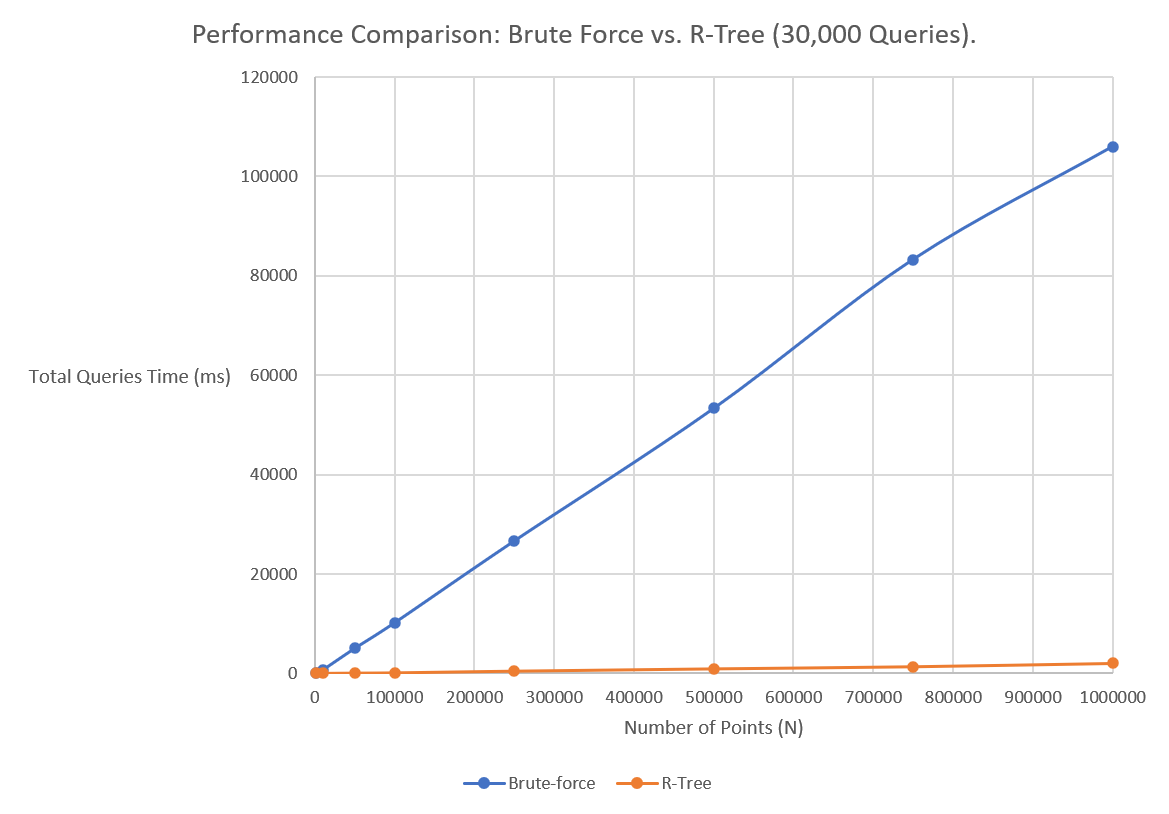
\includegraphics[width=0.9\textwidth]{time_chart.png}
    \caption{Execution time comparison between Brute-force and R-Tree}
\end{figure}

The chart clearly illustrates the difference in time complexity between the two algorithms when executing 30,000 queries. The Brute-force method exhibits linear growth $\mathcal{O}(N)$, leading to a sharp increase in running time, taking nearly 106 seconds (105,970 ms) to complete queries on a dataset of 1 million points. Conversely, the R-Tree structure proves its optimization through the spatial pruning mechanism with an asymptotic complexity of $\mathcal{O}(\log N)$. The query time of the R-Tree grows extremely slowly, taking only about 2 seconds (2026.34 ms) for the same data scale. At the $N = 1,000,000$ mark, the R-Tree achieves a speedup approximately 52 times faster than Brute-force, confirming the superior performance of indexing when handling a massive number of queries.

\vspace{1cm}

\section{2. Memory Usage Evaluation}

\begin{figure}[H]
    \centering
    % Thay "memory_chart.png" bằng tên file ảnh thực tế
    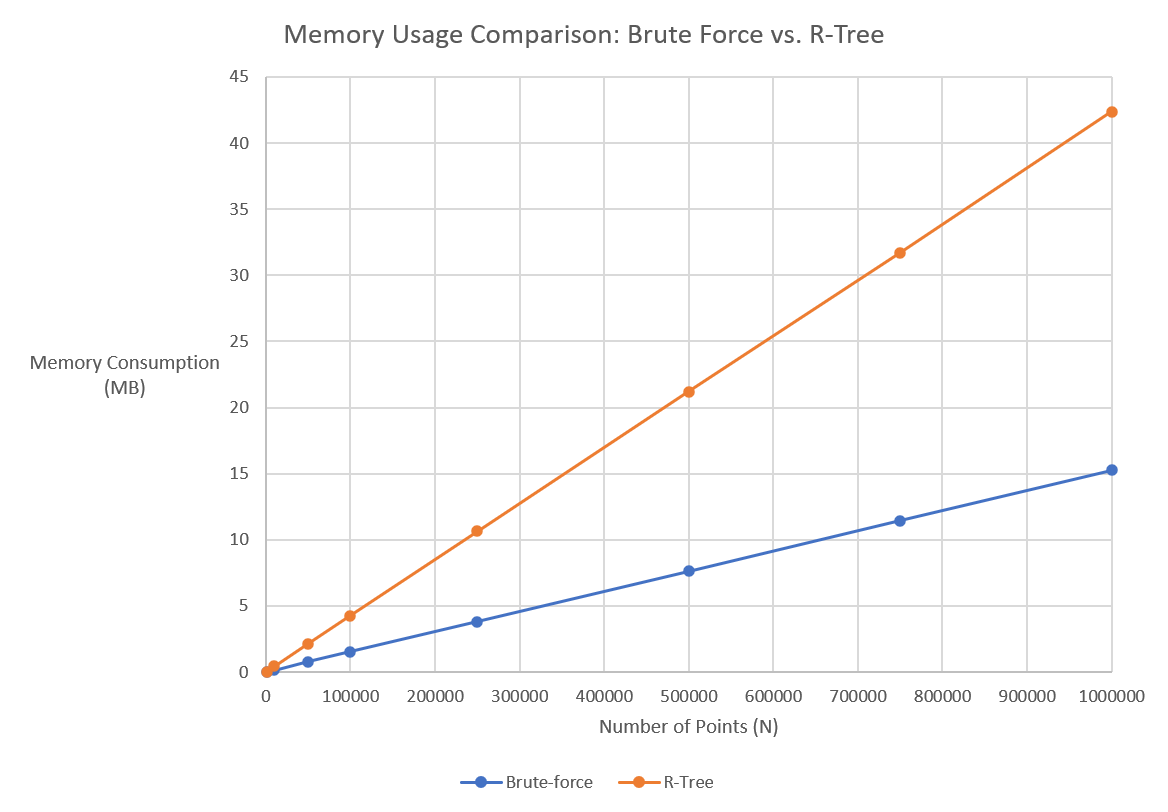
\includegraphics[width=0.9\textwidth]{memory_chart.png}
    \caption{Memory usage comparison between Brute-force and R-Tree}
\end{figure}

The chart demonstrates the mandatory trade-off in storage space to exchange for query speed. Both methods exhibit linear growth in RAM consumption according to the number of points. The Brute-force method perfectly optimizes space by only storing coordinates in an array (costing 15.26 MB for 1 million points). Meanwhile, the R-Tree consumes about 42.38 MB, which is 2.7 to 2.8 times higher than the linear array. This memory overhead arises because the system must allocate extra memory to maintain the hierarchical structure of the tree, including storing the coordinates of the Minimum Bounding Rectangles (MBRs) at internal nodes and the pointers linking parent and child nodes. Despite consuming more space, this is a completely worthwhile and feasible trade-off on modern computer systems.

\chapter{Implementation and Libraries}

% ==============================================================================
% 1. SOURCE CODES 
% ==============================================================================
\section{Source Codes}

The entire source code, including the header of the R-Tree data structure, the \texttt{main.cpp} file for performance evaluation (clearly displaying critical parameters and comparing directly with the brute-force algorithm), along with the Python source code, have been fully uploaded and organized into a complete repository.

Details on how to run (instructions) are clearly presented in the project's README file.

\textbf{Access the source code on GitHub:} \url{https://github.com/vbthg/R-tree}

% ==============================================================================
% 2. PRODUCTION-READY LIBRARY: BOOST.GEOMETRY
% ==============================================================================
\section{Production-Ready Implementation: Boost.Geometry}

While implementing an R-Tree from scratch is essential for understanding its underlying spatial pruning mechanics, industry applications typically rely on heavily optimized, battle-tested libraries to handle massive geographic datasets. In the C++ ecosystem, the industry standard for spatial indexing is the \texttt{boost::geometry::index::rtree} module from the widely acclaimed Boost C++ Libraries.

\subsection{Key Advantages and Features}
The Boost.Geometry R-Tree provides several distinct advantages that make it suitable for production environments:

\begin{itemize}
    \item \textbf{Multidimensional Data Support:} Unlike basic implementations restricted to 2D planes, Boost natively supports indexing in 2D, 3D, and even higher-dimensional spaces.
    \item \textbf{Algorithmic Flexibility:} It provides built-in support for various tree balancing algorithms out-of-the-box, allowing developers to choose between Linear, Quadratic, and the highly optimized R*-Tree (R-Star Tree) depending on the use case.
    \item \textbf{Header-only Integration:} It requires no complex linking processes or the compilation of separate \texttt{.dll} or \texttt{.lib} binaries. Developers simply include the headers, making it highly portable.
    \item \textbf{Generic Programming:} Built heavily on C++ templates, it can index any custom user-defined data type as long as the spatial properties are properly mapped.
    \item \textbf{Thread Safety:} Concurrent read queries (e.g., multiple users searching the map simultaneously) are completely thread-safe.
\end{itemize}

\subsection{Built-in Functions (API)}
The library encapsulates complex tree operations into a clean, easy-to-use API. The most commonly used built-in functions include:

\begin{itemize}
    \item \texttt{insert(Value const \&)}: Inserts a new spatial object into the tree, automatically handling node splitting if an overflow occurs.
    \item \texttt{remove(Value const \&)}: Removes a specific object and handles potential node underflows and tree condensation.
    \item \texttt{query(Predicate, OutIter)}: The core search function. It accepts powerful spatial predicates to filter data without writing manual loops:
    \begin{itemize}
        \item \texttt{bgi::intersects(Geometry)}: Finds all objects overlapping the query geometry (used for Window Queries).
        \item \texttt{bgi::within(Geometry)}: Finds all objects completely inside the query geometry.
        \item \texttt{bgi::nearest(Point, k)}: Finds the $k$ nearest neighbors (KNN) to a specific point.
    \end{itemize}
    \item \texttt{size()}: Returns the total number of elements currently stored in the R-Tree in $\mathcal{O}(1)$ time.
    \item \texttt{bounds()}: Returns the Minimum Bounding Rectangle (MBR) of the entire tree (i.e., the MBR of the root node).
    \item \texttt{clear()}: Completely removes all elements and frees the allocated memory.
\end{itemize}

\subsection{Installation and Integration}
Since the Boost.Geometry R-Tree is a \textbf{header-only} library, it does not require a pre-compiled binary. Developers only need to ensure the Boost headers are available in the compiler's search path.

\begin{enumerate}
    \item \textbf{Manual Installation:}
    \begin{itemize}
        \item Download the Boost source from \url{https://www.boost.org/}.
        \item Extract the archive and add the \texttt{/boost} subdirectory to your project's \texttt{Include} path in your IDE (e.g., Visual Studio, CLion, or VS Code).
    \end{itemize}
    \item \textbf{Package Managers (Recommended):}
    \begin{itemize}
        \item \textbf{Windows (vcpkg):} Run \texttt{vcpkg install boost-geometry} in the terminal.
        \item \textbf{Linux (Ubuntu/Debian):} Run \texttt{sudo apt-get install libboost-all-dev}.
        \item \textbf{macOS (Homebrew):} Run \texttt{brew install boost}.
    \end{itemize}
    \item \textbf{Linking:} No extra linking (\texttt{-l}) flags are required during compilation. Simply use \texttt{\#include <boost/geometry.hpp>} in your source files.
\end{enumerate}

\subsection{Basic Setup and Data Type Definition}
To utilize the R-Tree, we must first include the necessary headers and define our spatial geometries (Points and Boxes), along with the payload data we intend to store inside the tree.

\begin{verbatim}
#include <boost/geometry.hpp>
#include <boost/geometry/index/rtree.hpp>
#include <vector>
#include <iostream>

namespace bg = boost::geometry;
namespace bgi = boost::geometry::index;

// Define a 2D point using Cartesian coordinates
typedef bg::model::point<double, 2, bg::cs::cartesian> Point;
// Define a 2D box (MBR) using the Point type
typedef bg::model::box<Point> Box;
// Define the value type stored in the tree (e.g., an MBR and a Segment ID)
typedef std::pair<Box, int> Value;
\end{verbatim}

\subsection{Tree Initialization and Data Insertion}
Boost allows developers to specify the splitting heuristic at compile time. In the following example, we initialize an R-Tree using the Quadratic split algorithm with a maximum node capacity of 16 entries.

\begin{verbatim}
int main()
{
    // Initialize the R-Tree with a Quadratic splitting algorithm
    bgi::rtree< Value, bgi::quadratic<16> > rtree;

    // Create sample bounding boxes representing road segments
    Box box1(Point(0, 0), Point(2, 2));
    Box box2(Point(5, 5), Point(7, 7));
    Box box3(Point(1, 1), Point(3, 3));

    // Insert data into the R-Tree
    rtree.insert(std::make_pair(box1, 101));
    rtree.insert(std::make_pair(box2, 102));
    rtree.insert(std::make_pair(box3, 103));
\end{verbatim}

\subsection{Executing Spatial Queries}
The true power of the Boost R-Tree lies in its expressive and highly optimized querying capabilities, seamlessly supporting both orthogonal range reporting and proximity searches.

\textbf{1. Window Query (Intersection)} \\
This query is identical to the Filter Step in GIS map rendering, retrieving all segments that overlap with a defined viewing region.

\begin{verbatim}
    // Define the query window (e.g., the user's screen)
    Box screen_window(Point(1, 1), Point(4, 4));
    std::vector<Value> window_results;

    // Query: Find all items intersecting the screen_window
    rtree.query(bgi::intersects(screen_window), std::back_inserter(window_results));

    // Process the candidate set
    for(auto const& item : window_results)
    {
        if(item.second > 0)
        {
            std::cout << "Candidate Segment ID: " << item.second << std::endl;
        }
    }
\end{verbatim}

\textbf{2. K-Nearest Neighbors (KNN) Query} \\
This query finds a specified number of objects closest to a given geographical point, which is crucial for location-based services like finding nearby drivers.

\begin{verbatim}
    Point user_location(0, 0);
    std::vector<Value> knn_results;

    // Query: Find the 2 nearest items to the user_location
    rtree.query(bgi::nearest(user_location, 2), std::back_inserter(knn_results));

    for(auto const& item : knn_results)
    {
        std::cout << "Nearby Segment ID: " << item.second << std::endl;
    }

    return 0;
}
\end{verbatim}

% ==============================================================================
% 3. DATASETS
% ==============================================================================
\section{Datasets}

The large-scale datasets used to run the benchmark have been fully provided in the GitHub repository at the same link above.

\chapter{Programming Assignments}

\section{Exercise 1}
In a Geographic Information System (GIS) that manages road segments, we are given a list of thousands of line segments (roads) and a rectangular query window representing the user’s display screen. \\
The task is to find all road segments that need to be drawn on the screen.

\textbf{Solution:}

\textbf{Approach 1: Brute-force}
\begin{itemize}
    \item \textbf{Method:} Iterate through all $n$ line segments and check whether each segment intersects with the query rectangle.
    \item \textbf{Complexity:} $\mathcal{O}(n)$ per query, where $n$ is the total number of line segments.
    \item \textbf{Evaluation:} In practice, the system must answer numerous consecutive queries (as the user pans, zooms in/out of the map) $\rightarrow$ This approach is too slow and unfeasible.
\end{itemize}

\textbf{Approach 2: Applying the Filter and Refinement Framework with R-Tree}

Instead of checking everything, we filter out line segments located far from the query rectangle and only detail-check the "potential" segments. This process consists of 2 standard steps in commercial systems:

\textbf{Step 1: Filter Step}
\begin{itemize}
    \item \textbf{Create MBR:} Represent each line segment with a Minimum Bounding Rectangle (MBR). Formula: A line segment formed by 2 points $(x_1, y_1)$ and $(x_2, y_2)$ will have an MBR with the bottom-left corner at $(\min(x_1, x_2), \min(y_1, y_2))$ and the top-right corner at $(\max(x_1, x_2), \max(y_1, y_2))$.
    \item \textbf{R-Tree Query:} Insert all $n$ MBRs into the R-Tree. Using the R-Tree's Window Query algorithm, we quickly identify the MBRs that intersect with the query rectangle.
    \item \textbf{Result:} The set of line segments corresponding to the retrieved MBRs is called the Candidate set.
    \item \textbf{Complexity:} Using the R-Tree reduces the search cost to only $\mathcal{O}(\log n + k)$, where $k$ is the number of line segments in the candidate set. Since $k \ll n$, this operation eliminates most unnecessary data, speeding up the query thousands of times.
\end{itemize}

\textbf{Step 2: Refinement Step}
\begin{itemize}
    \item \textbf{Question:} Why do we still need to iterate and re-check after finding the candidate set?
    \item \textbf{Explanation:} This step is mandatory to eliminate False hits. This situation occurs when the MBR of a line segment intersects with the query window, but the actual line segment inside that MBR does not touch the query window at all.
    \item \textbf{Operation:} Scan through the candidate set (with a very small size $k$) and use a geometric algorithm to check the exact intersection between the line segment and the query window. The segments that truly intersect will be selected to be drawn on the screen.
\end{itemize}

\vspace{0.5cm}

\section{Exercise 2: Region Query on a Set of Rectangles}
Given a set $S$ consisting of rectangles with edges parallel to the coordinate axes. Given a query rectangle $r$, return all rectangles in $S$ that are covered by $r$.

\textbf{Solution:}

\textbf{1. Data Structure}
\begin{itemize}
    \item \textbf{Internal Node:} Stores Minimum Bounding Rectangles (MBRs) and pointers to child nodes.
    \item \textbf{Leaf Node:} Directly stores the coordinates of the data rectangles belonging to set $S$ (each rectangle is defined by 4 boundaries: left, right, top, bottom).
\end{itemize}

\textbf{2. Insertion \& Splitting}
\begin{itemize}
    \item \textbf{Choose Subtree:} When adding a new rectangle to the tree, traverse from the root downwards. At each internal node, choose the child branch whose MBR requires the least "perimeter enlargement" to fully enclose the new rectangle.
    \item \textbf{Overflow Handling:} When a leaf node exceeds its maximum capacity, it is mandatory to use an Internal-node Split Algorithm to split it in half. Reason: The data at the leaf node is now a rectangle (with area and 4 edges) rather than a point (1D coordinate). The algorithm will sort the list of rectangles sequentially by the left, right, top, and bottom boundaries along the X and Y axes. The system will try cutting at valid positions (ensuring each group has at least $0.4B$ elements) to find a split that minimizes the total perimeter of the 2 newly generated MBRs.
\end{itemize}

\textbf{3. Querying}

Start the recursive search function from the root node with the query rectangle $r$:
\begin{itemize}
    \item \textbf{Step 1 - Filtering at Internal Node:} Iterate through the child branches. Check whether the MBR of that child branch intersects or is covered by $r$.
    \begin{itemize}
        \item If yes: Recursively traverse down that branch.
        \item If no: Prune and completely skip that branch to save time.
    \end{itemize}
    \item \textbf{Step 2 - Checking at Leaf Node:} Upon reaching a leaf node, iterate through the stored data rectangles. Check the condition if the data rectangle lies completely inside $r$:
    \begin{itemize}
        \item Condition: \texttt{data.left >= r.left} AND \texttt{data.right <= r.right} AND \texttt{data.bottom >= r.bottom} AND \texttt{data.top <= r.top}.
        \item If all are satisfied, add that rectangle to the result list.
    \end{itemize}
\end{itemize}

\textbf{4. Complexity}
\begin{itemize}
    \item The average search cost is reduced to $\mathcal{O}(\log n + k)$, where $n$ is the total number of rectangles in the tree and $k$ is the number of rectangles within the region $r$ (the returned results).
\end{itemize}

\vspace{0.5cm}

\section{Exercise 3: K-Nearest Neighbors (KNN)}
\textbf{Problem Statement:} Given a set $S$ of $N$ data points on a 2D plane indexed by an R-Tree. Given a query point $P$ and a positive integer $K$. Find $K$ points in $S$ that have the shortest Euclidean distance to $P$.

\textbf{Detailed Solution:}

Instead of a Window Query like the previous exercises, the KNN problem uses the Best-First Search algorithm combined with a Priority Queue (Min-Heap) to traverse the R-Tree.

\textbf{1. Core Concept: Minimum Distance (MinDist)}
\begin{itemize}
    \item For the algorithm to know which branch to descend first, we must calculate the distance from the query point $P$ to the MBRs of the R-Tree.
    \item MinDist(P, MBR) is the shortest distance from point $P$ to any point lying on the boundary or inside that MBR.
    \item If $P$ lies completely inside the MBR, MinDist = 0. Thanks to MinDist, we can sort and prioritize opening the branches most likely to contain the points closest to $P$.
\end{itemize}

\textbf{2. Algorithm Execution Steps:}
\begin{itemize}
    \item \textbf{Step 1 (Initialization):} Create a Priority Queue (Min-Heap) to store the nodes of the R-Tree, sorted in ascending order by MinDist value. Initially, push the root node of the R-Tree into the queue. Create an empty list to store the $K$ results.
    \item \textbf{Step 2 (Traversing Min-Heap):} Repeat the following process until the queue is empty or $K$ result points have been collected: Extract the element with the smallest MinDist from the top of the queue.
    \item \textbf{Step 3 (Processing the extracted element):}
    \begin{itemize}
        \item \textbf{Case A (It is an actual data point):} Since it was extracted from the Min-Heap, it is certainly the closest point to $P$ currently. Add this point to the result list. If the list has enough $K$ elements, the algorithm terminates.
        \item \textbf{Case B (It is an internal node / MBR):} This node contains child branches. Calculate the MinDist from $P$ to all child MBRs (or child points) of that node. Push all these children back into the Min-Heap. The algorithm automatically resorts so the closest element always bubbles to the top.
    \end{itemize}
\end{itemize}

\textbf{3. Complexity Evaluation:}
\begin{itemize}
    \item This algorithm is highly optimal because it exploits the "pruning" property of the R-Tree. MBRs located too far from $P$ will have a very large MinDist, sink to the bottom of the Min-Heap, and almost never be extracted for traversal (avoiding scanning all $N$ points).
    \item The average complexity of this query is $\mathcal{O}(\log N + K)$.
\end{itemize}

\vspace{0.5cm}

\section{Exercise 4: Point Enclosure Query (Application in Mouse Click Detection on UI)}
\textbf{Problem Statement:}
In User Interface (UI) programming, components like panels, windows, or buttons are often represented by Bounding Boxes and can overlap. Given a set $S$ consisting of $N$ rectangles representing UI components. Given $Q$ queries, each corresponding to a mouse click at coordinates $P(x, y)$. Find all rectangles in $S$ that enclose point $P$.

\textbf{Detailed Solution:}

\textbf{Approach 1: Brute-force}
\begin{itemize}
    \item \textbf{Method:} For each point $P(x, y)$, iterate through all $N$ rectangles. Point $P$ is considered inside the rectangle if its coordinates satisfy the condition: $x_{min} \le x \le x_{max}$ and $y_{min} \le y \le y_{max}$.
    \item \textbf{Complexity:} $\mathcal{O}(N)$ per query. If the system has a large number of UI elements or complex polygons, this method will cause latency during user interaction.
\end{itemize}

\textbf{Approach 2: Applying R-Tree}

This problem is the inverse of Exercise 2. Instead of using a region to find objects inside it, we use a point to find the regions covering it.
\begin{itemize}
    \item \textbf{Data Structure:} Build an R-Tree where the leaf nodes store the coordinates of the $N$ UI rectangles.
    \item \textbf{Query Operation:} A recursive search function starting from the root node:
    \begin{itemize}
        \item \textbf{At the Internal Node:} For each child branch, check whether point $P(x, y)$ lies inside the MBR of that branch.
        \begin{itemize}
            \item If $P$ is not inside the MBR, $P$ definitely cannot be inside any element belonging to that branch $\rightarrow$ Completely prune this branch.
            \item If $P$ is inside the MBR, recursively traverse down the child branch.
        \end{itemize}
        \item \textbf{At the Leaf Node:} Scan through the stored data rectangles. Check whether point $P$ truly lies inside that rectangle (checking 4 boundaries). If yes, add this rectangle to the result list.
    \end{itemize}
    \item \textbf{Complexity:} By pruning irrelevant UI areas, the R-Tree narrows down the search scope extremely fast. The average time to process each mouse click drops to $\mathcal{O}(\log N + k)$, where $k$ is the number of UI components overlapping at the exact coordinate $P$. The interaction response process occurs in approximately $\mathcal{O}(1)$ in practice.
\end{itemize}

\newpage


\newpage
% ==============================================================================
% 4. PERFORMANCE COMPARISON
% ==============================================================================


\begin{thebibliography}{9}

\bibitem{guttman84}
Antonin Guttman. 
\textit{R-Trees: A Dynamic Index Structure for Spatial Searching}. 
Proceedings of the 1984 ACM SIGMOD International Conference on Management of Data, pp. 47–57, 1984[cite: 833].
\textit{Source: http://db.deis.unibo.it/courses/SI-LS/papers/Gut84.pdf}

\bibitem{tao_course}
Yufei Tao. 
\textit{The R-Tree}. 
Lecture Notes for INFS4205/7205, University of Queensland[cite: 2, 5].
\textit{Source: https://www.cse.cuhk.edu.hk/~taoyf/course/infs4205/lec/rtree.pdf}

\bibitem{tao_notes}
Yufei Tao. 
\textit{Spatial Databases - Lecture 13: R-Tree}. 
Course Notes, The Chinese University of Hong Kong.
\textit{Source: https://www.cse.cuhk.edu.hk/~taoyf/course/wst501/notes/lec13.pdf}

\bibitem{gatech_slides}
Joyeeta Arulraj. 
\textit{Database Systems Implementation - Lecture 17: R-Trees}. 
Georgia Institute of Technology, Fall 2024.
\textit{Source: https://faculty.cc.gatech.edu/~jarulraj/courses/4420-f24/slides/17-rtree.pdf}

\end{thebibliography}

\end{document}